\documentclass[UTF8,a4paper,12pt]{ctexbook} 

\usepackage{graphicx}%学习插入图
\usepackage{verbatim}%学习注释多行
\usepackage{booktabs}%表格
\usepackage{geometry}%图片
\usepackage{amsmath}
\usepackage{amssymb}
\usepackage{listings}%代码
\usepackage{xcolor}  %颜色
\usepackage{enumitem}%列表格式
\setenumerate[1]{itemsep=0pt,partopsep=0pt,parsep=\parskip,topsep=5pt}
\setitemize[1]{itemsep=0pt,partopsep=0pt,parsep=\parskip,topsep=5pt}
\setdescription{itemsep=0pt,partopsep=0pt,parsep=\parskip,topsep=5pt}
\usepackage{tcolorbox}
\usepackage{algorithm}  %format of the algorithm
\usepackage{algorithmic}%format of the algorithm
\usepackage{multirow}   %multirow for format of table
\usepackage{tabularx} 	%表格排版格式控制
\usepackage{array}	%表格排版格式控制
\usepackage{hyperref} %超链接 \url{URL}

\CTEXsetup[format+={\flushleft}]{section}

%%%% 设置图片目录
\graphicspath{{figure/}}

%%%% 段落首行缩进两个字 %%%%
\makeatletter
\let\@afterindentfalse\@afterindenttrue
\@afterindenttrue
\makeatother
\setlength{\parindent}{2em}  %中文缩进两个汉字位

%%%% 下面的命令重定义页面边距,使其符合中文刊物习惯 %%%%
\addtolength{\topmargin}{-54pt}
\setlength{\oddsidemargin}{0.63cm}  % 3.17cm - 1 inch
\setlength{\evensidemargin}{\oddsidemargin}
\setlength{\textwidth}{14.66cm}
\setlength{\textheight}{24.00cm}    % 24.62

%%%% 下面的命令设置行间距与段落间距 %%%%
\linespread{1.4}
\setlength{\parskip}{0.5\baselineskip}
\geometry{left=1.6cm,right=1.8cm,top=2cm,bottom=1.7cm} %设置文章宽度
\pagestyle{plain} 		  %设置页面布局

%代码效果定义
\definecolor{mygreen}{rgb}{0,0.6,0}
\definecolor{mygray}{rgb}{0.5,0.5,0.5}
\definecolor{mymauve}{rgb}{0.58,0,0.82}
\lstset{ %
	backgroundcolor=\color{white},   % choose the background color
	basicstyle=\footnotesize\ttfamily,      % size of fonts used for the code
	%stringstyle=\color{codepurple},
	%basicstyle=\footnotesize,
	%breakatwhitespace=false,         
	%breaklines=true,                 
	%captionpos=b,                    
	%keepspaces=true,                 
	%numbers=left,                    
	%numbersep=5pt,                  
	%showspaces=false,                
	%showstringspaces=false,
	%showtabs=false,        
	columns=fullflexible,
	breaklines=true,                 % automatic line breaking only at whitespace
	captionpos=b,                    % sets the caption-position to bottom
	tabsize=4,
	commentstyle=\color{mygreen},    % comment style
	escapeinside={\%*}{*)},          % if you want to add LaTeX within your code
	keywordstyle=\color{blue},       % keyword style
	stringstyle=\color{mymauve}\ttfamily,     % string literal style
	frame=single,
	rulesepcolor=\color{red!20!green!20!blue!20},
	% identifierstyle=\color{red},
	language=c++,
}
 \author{\kaishu 郑华}
 \title{\heiti CUDA笔记}
 
\begin{document}          %正文排版开始
 	\maketitle
	\tableofcontents
	
\chapter{入门}
	\section{参考}\url{http://blog.chinaunix.net/uid-20620288-id-4705367.html} \\
	
	\url{http://bbs.csdn.net/topics/390798229}
	
	\section{CUDA 简介}
		\textbf{CUDA},\verb|Compute Unified Device Architecture|的简称,是由\verb|NVIDIA|公司创立的基于他们公司生产的图形处理器\verb|GPUs|(\verb|Graphics Processing Units|,可以通俗的理解为显卡)的一个并行计算平台和编程模型。
		通过\verb|CUDA|,\verb|GPUs|可以很方便地被用来进行通用计算(有点像在\verb|CPU|中进行的数值计算等等)。在没有\verb|CUDA|之前,\verb|GPUs|一般只用来进行图形渲染(如通过\verb|OpenGL,DirectX|)。
		
		开发人员可以通过调用\verb|CUDA|的\verb|API|,来进行并行编程,达到高性能计算目的。\verb|NVIDIA|公司为了吸引更多的开发人员,对\verb|CUDA|进行了编程语言扩展,如\verb|CUDA C/C++,CUDA Fortran|语言。注意\verb|CUDA C/C++|可以看作一个新的编程语言,因为\verb|NVIDIA|配置了相应的编译器\verb|nvcc|
	
	\section{基本概念}
		\subsection{主机}
			将\verb|CPU|及系统的内存(内存条)称为主机
			
		\subsection{设备}
			将\verb|GPU|及\verb|GPU|本身的显示内存称为设备,设备中分为大核和小核, 流多处理器,大核是也, 小核则是线程并行单元流处理器。
			
		\subsection{线程}
			 一般通过GPU的一个核进行处理。(可以表示成一维,二维,三维)
			 
		\subsection{线程块}
			\begin{enumerate}
				\item 由多个线程组成
				\item 各\verb|block|是并行执行的,\verb|block|间无法通信,也没有执行顺序
				\item 注意线程块的数量限制为不超过\verb|65535|(硬件限制)。
			\end{enumerate}
			
		\subsection{线程格}
			由多个线程块组成.
			
			\begin{figure}[h]
				\centering
				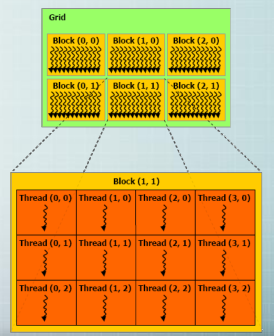
\includegraphics[scale = 1.2]{ThreadCUDA.png}
			\end{figure}
			
		\subsection{线结束}
			在\verb|CUDA|架构中,线程束是指一个包含32个线程的集合,这个线程集合被“编织在一起”并且“步调一致”的形式执行。在程序中的每一行,线程束中的每个线程都将在不同数据上执行相同的命令。
		
		\subsection{函数修饰符}	
			\begin{enumerate}
				\item \verb|__global__ |表明被修饰的函数\textbf{在设备上执行,但在主机上调用}	
				\item \verb|__device__ |表明被修饰的函数\textbf{在设备上执行},但只能在其他\verb|__device__|函数或者\verb|__global__|函数中调用
			\end{enumerate}

		\subsection{核函数}
			\begin{enumerate}
				\item 在GPU上执行的函数通常称为核函数
				\item 一般通过标识符\verb|__global__|修饰,调用通过\verb|<<<参数1,参数2>>>|,用于说明内核函数中的线程数量,以及线程是如何组织的。
				\item 以线程格(\verb|Grid|)的形式组织,每个线程格由若干个线程块(\verb|block|)组成,而每个线程块又由若干个线程(\verb|thread|)组成
				\item 是以\verb|block|为单位执行的
				\item 叧能在主机端代码中调用
				\item 调用时必须声明内核函数的执行参数
				\item 在编程时,必须先为kernel函数中用到的数组或变量分配好足够的空间,再调用kernel函数,否则在GPU计算时会发生错误,例如越界或报错,甚至导致蓝屏和死机
				
				\begin{lstlisting}
	/*
	* @file_name HelloWorld.cu  后缀名称.cu
	*/
	
	#include <stdio.h>
	#include <cuda_runtime.h>  //头文件
	
	//核函数声明,前面的关键字__global__
	__global__ void kernel( void ) {}
	
	int main( void ) {
		//核函数的调用,注意<<<1,1>>>,第一个1,代表线程格里只有一个线程块;第二个1,代表一个线程块里只有一个线程。
		kernel<<<1,1>>>();
		printf( "Hello, World!\n" );
		return 0;
	}
				\end{lstlisting}
			\end{enumerate}
		\subsection{dim3结构类型}
			\begin{enumerate}
				\item \verb|dim3|是基亍\verb|uint3|定义的矢量类型,相当亍由3个\verb|unsigned int|型组成的结构体。\verb|uint3|类型有三个数据成员\verb|unsigned int x|; \verb|unsigned int y|; \verb|unsigned int z|;
				\item 可使用亍一维、二维或三维的索引来标识线程,构成一维、二维或三维线程块。
				\item \verb|dim3|结构类型变量用在核函数调用的\verb|<<<,>>>|中
				\item 相关的几个内置变量
					\begin{itemize}
						\item \verb|threadIdx|,顾名思义获取线程\verb|thread|的\verb|ID|索引;如果线程是一维的那么就取 \verb|threadIdx.x|,二维的还可以多取到一个值 \verb|threadIdx.y|,以此类推到三维 \verb|threadIdx.z|
						\item \verb|blockIdx,|线程块的\verb|ID|索引;同样有 \verb|blockIdx.x,blockIdx.y,blockIdx.z|
						\item \verb|blockDim|,线程块的维度,同样有 \verb|blockDim.x,blockDim.y,blockDim.z|
						\item \verb|gridDim|,线程格的维度,同样有 \verb|gridDim.x,gridDim.y,gridDim.z|
					\end{itemize}
				\item 对于一维的\verb|block|,线程的 \verb|threadID| \verb|= threadIdx.x|
				\item 对于大小为(\verb|blockDim.x, blockDim.y|)的 二维 \verb|block|,线程的 \verb|threadID| \verb|= threadIdx.x| +\verb| threadIdx.y*blockDim.x|
				\item 对于大小为(\verb|blockDim.x, blockDim.y, blockDim.z|)的 三维 \verb|block|,线程的 \verb|threadID| \verb|= threadIdx.x+threadIdx.y*blockDim.x+threadIdx.z*blockDim.x*blockDim.y|
				
				\item 对于计算线程索引偏移增量为已启动线程的总数。如 \verb|stride| \verb|= blockDim.x * gridDim.x;| \verb|threadId += stride|
			\end{enumerate}

\chapter{进阶}
	\section{常用的GPU函数}
		\subsection{cudaMalloc()}
			\subparagraph{函数原型} \verb|cudaError_t cudaMalloc (void **devPtr, size_t size)|
			\subparagraph{函数用处} 与C语言中的\verb|malloc|函数一样,只是此函数在GPU的内存你分配内存
			\subparagraph{注意事项}
				\begin{enumerate}[itemindent = 1em]
					\item 可以将\verb|cudaMalloc()|分配的指针传递给在设备上执行的函数
					\item 可以在设备代码中使用\verb|cudaMalloc()|分配的指针进行设备内存读写操作
					\item 可以将\verb|cudaMalloc()|分配的指针传递给在主机上执行的函数
					\item 不可以在主机代码中使用\verb|cudaMalloc()|分配的指针进行主机内存读写操作(即不能进行解引用)。
				\end{enumerate}
				
		\subsection{cudaMemcpy()}
			\subparagraph{函数原型} \verb|cudaError_t  cudaMemcpy (void *dst, const void *src, size_t count,| \verb|cudaMemcpyKind| \verb| kind)|
			\subparagraph{函数用处} 与c语言中的\verb|memcpy|函数一样,只是此函数可以在主机内存和\verb|GPU|内存之间互相拷贝数据
			\subparagraph{函数参数} \verb|cudaMemcpyKind kind|表示数据拷贝方向,如果kind赋值为\verb|cudaMemcpyDeviceToHost|表示数据从设备内存拷贝到主机内存		
			\subparagraph{其他}
				\begin{enumerate}[itemindent = 1em]
					\item 与C中的\verb|memcpy()|一样,以同步方式执行,即当函数返回时,复制操作就已经完成了,并且在输出缓冲区中包含了复制进去的内容
					\item 相应的有个异步方式执行的函数\verb|cudaMemcpyAsync()|,这个函数详解请看下面的流一节有关内容
				\end{enumerate}
			
		\subsection{cudaFree()}
			\subparagraph{函数原型}\verb|cudaError_t cudaFree ( void* devPtr )|
			\subparagraph{函数作用}与c语言中的\verb|free()|函数一样,只是此函数释放的是\verb|cudaMalloc()|分配的内存
			
		\subsection{示例}
			\begin{lstlisting}
	#include <stdio.h>
	#include <cuda_runtime.h>
	__global__ void add( int a, int b, int *c ) {
		*c = a + b;
	}
	int main( void ) {
		int c;
		int *dev_c;
		//cudaMalloc()
		cudaMalloc( (void**)&dev_c, sizeof(int) );
		//核函数执行
		add<<<1,1>>>( 2, 7, dev_c );   
		//cudaMemcpy()
		cudaMemcpy( &c, dev_c, sizeof(int),cudaMemcpyDeviceToHost ) ;
		printf( "2 + 7 = %d\n", c );
		//cudaFree()
		cudaFree( dev_c );
		
		return 0;
	}
			\end{lstlisting}
	
	\section{GPU内存分类}
		\subsection{全局内存}
			通俗意义上的 \textbf{设备内存}
		\subsection{共享内存}
			\subparagraph{位置}设备内存
			\subparagraph{形式}关键字\verb|__shared__|添加到变量声明中。如\verb|__shared__ float cache[10]|
			\subparagraph{目的}对于\verb|GPU|上启动的每个线程块,\verb|CUDA C|编译器都将创建该共享变量的一个副本。\textbf{线程块中的}每个线程都共享这块内存,\textbf{但线程却无法看到也不能修改其他线程块的变量副本}。这样使得一个线程块中的多个线程能够在计算上通信和协作
			
		\subsection{常量内存}
			\subparagraph{位置}设备内存
			\subparagraph{形式}关键字\verb|__constant__|添加到变量声明中。如\verb|__constant__ float s[10];|
			\subparagraph{目的}为了提升性能。常量内存采取了不同于标准全局内存的处理方式。在某些情况下,用常量内存替换全局内存能有效地减少内存带宽
			\subparagraph{特点}常量内存用于保存在核函数执行期间不会发生变化的数据。\textbf{变量的访问限制为只读}。NVIDIA硬件提供了\verb|64KB|的常量内存。不再需要\verb|cudaMalloc()或者cudaFree()|,而是在编译时,静态地分配空间
			\subparagraph{要求}当我们需要拷贝数据到常量内存中应该使用\verb|cudaMemcpyToSymbol()|,而\verb|cudaMemcpy()|会复制到全局内存
			
		\subsection{纹理内存}
			\subparagraph{位置}设备内存
			\subparagraph{目的}能够减少对内存的请求并提供高效的内存带宽。是专门为那些在内存访问模式中存在大量空间局部性的图形应用程序设计,意味着一个线程读取的位置可能与邻近线程读取的位置“非常接近”。如下图:
				\begin{figure}[h]
					\centering
					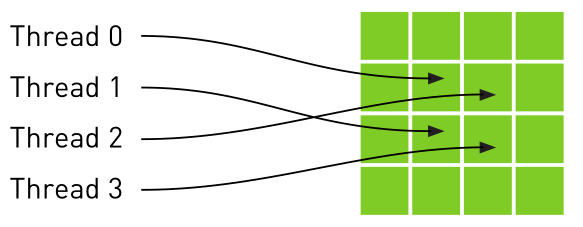
\includegraphics[scale = 0.7]{TextureMem.png}
				\end{figure}
				
		\subsection{固定内存}
			\subparagraph{位置}主机内存
			\subparagraph{概念}也称为页锁定内存或者不可分页内存,操作系统将不会对这块内存分页并交换到磁盘上,从而确保了该内存始终驻留在物理内存中。因此操作系统能够安全地使某个应用程序访问该内存的物理地址,因为这块内存将不会破坏或者重新定位。
			
			\subparagraph{目的}提高访问速度。由于GPU知道主机内存的物理地址,因此可以通过“直接内存访问\verb|DMA(Direct Memory Access)|技术来在GPU和主机之间复制数据。由于\verb|DMA|在执行复制时无需CPU介入。因此DMA复制过程中使用固定内存是非常重要的
			
			\subparagraph{形式}通过\verb|cudaHostAlloc()|函数来分配;通过\verb|cudaFreeHost()|释放
		
		\subsection{原子性}
			\subparagraph{概念}如果操作的执行过程不能分解为更小的部分,我们将满足这种条件限制的操作称为原子操作
			
			\subparagraph{形式}函数调用,如\verb|atomicAdd(addr,y)|将生成一个原子的操作序列,这个操作序列包括读取地址\verb|addr|处的值,将y增加到这个值,以及将结果保存回地址\verb|addr|。
			
			\url{http://www.opengpu.org/forum.php?mod=viewthread&tid=14715}
	
	\section{使用事件测试性能}
		\subparagraph{用途}为了测量\verb|GPU|在某个任务上花费的时间。\verb|CUDA|中的事件本质上是一个\verb|GPU|时间戳。由于事件是直接在\verb|GPU|上实现的。因此不适用于对同时包含设备代码和主机代码的混合代码设计
		
		\subparagraph{形式}首先创建一个事件,然后记录事件,再计算两个事件之差,最后销毁事件。如:
			\begin{lstlisting}
	cudaEvent_t start, stop;
	cudaEventCreate( &start );
	cudaEventCreate( &stop );
	cudaEventRecord( start, 0 );
	
	//do something
	
	cudaEventRecord( stop, 0 );
	float   elapsedTime;
	cudaEventElapsedTime( &elapsedTime,start, stop );
	cudaEventDestroy( start );
	cudaEventDestroy( stop );
			\end{lstlisting}
		
						
	\section{线程并行}
		多线程我们应该都不陌生,在操作系统中,进程是资源分配的基本单元,而线程是\verb|CPU|时间调度的基本单元(这里假设只有1个\verb|CPU|)。 
		
		将线程的概念引申到\verb|CUDA|程序设计中,我们可以认为线程就是执行\verb|CUDA|程序的最小单元,前面我们建立的工程代码中,有个核函数概念不知各位童鞋还记得没有,在\verb|GPU|上\textbf{每个线程}\underline{都会运行一次该核函数}。 
		
		但\verb|GPU|上的线程调度方式与\verb|CPU|有很大不同。\verb|CPU|上会有优先级分配,从高到低,同样优先级的可以采用时间片轮转法实现线程调度。\verb|GPU|上线程没有优先级概念,\textbf{所有线程机会均等},线程状态只有等待资源和执行两种状态,如果资源未就绪,那么就等待;一旦就绪,立即执行。当\verb|GPU|资源很充裕时,所有线程都是并行执行的,这样加速效果很接近理论加速比;而\verb|GPU|资源少于总线程个数时,有一部分线程就会等待前面执行的线程释放资源,从而变为串行化执行。 
		
		\begin{lstlisting}
	cudaError_t addWithCuda(int *c, const int *a, const int *b, size_t size);   
	__global__ void addKernel(int *c, const int *a, const int *b)   
	{   
		int i = threadIdx.x;   
		c[i] = a[i] + b[i];   
	}   
	int main()   
	{   
		const int arraySize = 5;   
		const int a[arraySize] = { 1, 2, 3, 4, 5 };   
		const int b[arraySize] = { 10, 20, 30, 40, 50 };   
		int c[arraySize] = { 0 };   
		// Add vectors in parallel.   
		cudaError_t cudaStatus;   
		int num = 0;   
		cudaDeviceProp prop;   
		cudaStatus = cudaGetDeviceCount(&num);   
		for(int i = 0;i 
		{   
			cudaGetDeviceProperties(&prop,i);   
		}   
		cudaStatus = addWithCuda(c, a, b, arraySize);   
		if (cudaStatus != cudaSuccess)    
		{   
			fprintf(stderr, "addWithCuda failed!");   
			return 1;   
		}   
		
		printf("{1,2,3,4,5} + {10,20,30,40,50} = {%d,%d,%d,%d,%d}\n",c[0],c[1],c[2],c[3],c[4]);   
		// cudaThreadExit must be called before exiting in order for profiling and   
		// tracing tools such as Nsight and Visual Profiler to show complete traces.   
		cudaStatus = cudaThreadExit();  
		 
		if (cudaStatus != cudaSuccess)    
		{   
			fprintf(stderr, "cudaThreadExit failed!");   
			return 1;   
		}   
		return 0;   
	}   
	
	// 重点理解这个函数   
	cudaError_t addWithCuda(int *c, const int *a, const int *b, size_t size)   
	{   
		int *dev_a = 0; //GPU设备端数据指针   
		int *dev_b = 0;   
		int *dev_c = 0;   
		cudaError_t cudaStatus;   //状态指示   
		
		// Choose which GPU to run on, change this on a multi-GPU system.   
		cudaStatus = cudaSetDevice(0);  //选择运行平台   
		if (cudaStatus != cudaSuccess)    
		{   
			fprintf(stderr, "cudaSetDevice failed!  Do you have a CUDA-capable GPU installed?");   
			goto Error;   
		}   
		// 分配GPU设备端内存   
		cudaStatus = cudaMalloc((void**)&dev_c, size * sizeof(int));   
		if (cudaStatus != cudaSuccess)    
		{   
			fprintf(stderr, "cudaMalloc failed!");   
			goto Error;   
		}   
		cudaStatus = cudaMalloc((void**)&dev_a, size * sizeof(int));   
		if (cudaStatus != cudaSuccess)    
		{   
			fprintf(stderr, "cudaMalloc failed!");   
			goto Error;   
		}   
		cudaStatus = cudaMalloc((void**)&dev_b, size * sizeof(int));   
		if (cudaStatus != cudaSuccess)    
		{   
			fprintf(stderr, "cudaMalloc failed!");   
			goto Error;   
		}   
		// 拷贝数据到GPU   
		cudaStatus = cudaMemcpy(dev_a, a, size * sizeof(int), cudaMemcpyHostToDevice);   
		if (cudaStatus != cudaSuccess)    
		{   
			fprintf(stderr, "cudaMemcpy failed!");   
			goto Error;   
		}   
		cudaStatus = cudaMemcpy(dev_b, b, size * sizeof(int), cudaMemcpyHostToDevice);   
		if (cudaStatus != cudaSuccess)    
		{   
			fprintf(stderr, "cudaMemcpy failed!");   
			goto Error;   
		}   
		// 运行核函数   
	    addKernel<<<1, size>>>(dev_c, dev_a, dev_b);  
	     
		// cudaThreadSynchronize waits for the kernel to finish, and returns   
		// any errors encountered during the launch.   
		cudaStatus = cudaThreadSynchronize();   //同步线程   
		
		if (cudaStatus != cudaSuccess)    
		{   
			fprintf(stderr, "cudaThreadSynchronize returned error code %d after launching addKernel!\n", cudaStatus);   
			goto Error;   
		}   
		// Copy output vector from GPU buffer to host memory.   
		cudaStatus = cudaMemcpy(c, dev_c, size * sizeof(int), cudaMemcpyDeviceToHost);      //拷贝结果回主机   
		if (cudaStatus != cudaSuccess)    
		{   
			fprintf(stderr, "cudaMemcpy failed!");   
			goto Error;   
		}   
		Error:   
			cudaFree(dev_c);    //释放GPU设备端内存   
			cudaFree(dev_a);   
			cudaFree(dev_b);       
		return cudaStatus;   
	} 
		\end{lstlisting}
		
	\verb|<<<>>>|表示运行时配置符号,里面1表示只分配一个线程组(又称线程块、\verb|Block|),\verb|size|表示每个线程组有\verb|size|个线程(\verb|Thread|)。
	
	本程序中\verb|size|根据前面传递参数个数应该为5,所以运行的时候,核函数在5个GPU线程单元上分别运行了一次,总共运行了5次。
	
	这5个线程是如何知道自己“身份”的?是靠\verb|threadIdx|这个内置变量,它是个dim3类型变量,接受\verb|<<<>>>|中第二个参数,它包含\verb|x,y,z| 3维坐标,而我们传入的参数只有一维,所以只有x值是有效的。通过核函数中\verb|int i = threadIdx.x|;这一句,每个线程可以获得自身的\verb|id|号,从而找到自己的任务去执行。
	
	
	\section{块并行}
		块并行相当于操作系统中多进程的情况,上节说到,\verb|CUDA|有线程组(线程块)的概念,将一组线程组织到一起,共同分配一部分资源,然后内部调度执行。\textbf{线程块与线程块之间,毫无瓜葛}。这有利于做更粗粒度的并行。我们将上一节的代码改为块并行版本如下:
			
			\begin{lstlisting}
		__global__ void addKernel(int *c, const int *a, const int *b)   
		{   
			int i = blockIdx.x;   
			c[i] = a[i] + b[i];   
		}   
		
		addKernel<<>>(dev_c, dev_a, dev_b);
			\end{lstlisting}
		
		和上一节相比,只有这两行有改变,\verb|<<<>>>|里第一个参数改成了\verb|size|,第二个改成了1,表示我们分配\verb|size|个线程块,每个线程块仅包含1个线程,总共还是有5个线程。这5个线程相互独立,执行核函数得到相应的结果,与上一节不同的是,每个线程获取\verb|id|的方式变为\verb|int i = blockIdx.x|;这是线程块\verb|ID|。	  
	
		\subsection{线程并行月块并行的区别}
			线程并行是细粒度并行,调度效率高;块并行是粗粒度并行,每次调度都要重新分配资源,有时资源只有一份,那么所有线程块都只能排成一队,串行执行。 
			
			我们的任务有时可以采用分治法,将一个大问题分解为几个小规模问题,将这些小规模问题分别用一个线程块实现,线程块内可以采用细粒度的线程并行,而块之间为粗粒度并行,这样可以充分利用硬件资源,降低线程并行的计算复杂度。适当分解,降低规模,在一些矩阵乘法、向量内积计算应用中可以得到充分的展示
		  
	\section{线程格并行-流}
		多个线程块组织成了一个\verb|Grid|,称为线程格。一组线程并行处理可以组织为一个\verb|block|,而一组\verb|block|并行处理可以组织为一个\verb|Grid|,很自然地想到,\verb|Grid|只是一个网格,我们是否可以利用多个网格来完成并行处理呢?答案就是利用流
	
		\textbf{流}可以实现在一个设备上\textbf{运行多个核函数}。前面的块并行也好,线程并行也好,运行的\textbf{核函数都是相同的}(代码一样,传递参数也一样)。而流并行,可以执行不同的核函数,也可以实现对同一个核函数传递不同的参数,实现任务级别的并行。
		
		\verb|CUDA|中的流用\verb|cudaStream_t|类型实现,用到的\verb|API|有以下几个:
		
		\verb|cudaStreamCreate(cudaStream_t *s)|用于创建流,
		
		\verb|cudaStreamDestroy(cudaStream_t s)|用于销毁流,
		
		\verb|cudaStreamSynchronize()|用于单个流同步,
		
		\verb|cudaDeviceSynchronize()|用于整个设备上的所有流同步,
		
		\verb|cudaStreamQuery()|用于查询一个流的任务是否已经完成
		
			\begin{lstlisting}
	cudaStream_t stream[5];   
	for(int i = 0;i<5;i++)   
	{   
		cudaStreamCreate(&stream[i]);   //创建流   
	}  
	
	for(int i = 0;i<5;i++)   
	{   
		// 线程块数 线程数 共享内存  流对象
		addKernel<<<1,1,0,stream[i]>>>(dev_c+i, dev_a+i, dev_b+i);    //执行流   
	}    
	
	for(int i = 0;i<5;i++)   
	{   
		cudaStreamDestroy(stream[i]);   //销毁流   
	}   
			\end{lstlisting}
		
		函数代码仍然和块并行的版本一样,只是在调用时做了改变,\verb|<<<>>>|中的参数多了两个,其中前两个和块并行、线程并行中的意义相同,仍然是\textbf{线程块数}(这里为1)、每个线程块中\textbf{线程数}(这里也是1)。第三个为0表示每个\verb|block|用到的\textbf{共享内存}大小,这个我们后面再讲;第四个为\textbf{流对象},表示当前核函数在哪个流上运行。
		
		我们创建了5个流,每个流上都装载了一个核函数,同时传递参数有些不同,也就是每个核函数作用的对象也不同。这样就实现了任务级别的并行,\textbf{当我们有几个互不相关的任务时},可以写多个核函数,资源允许的情况下,我们将这些核函数装载到不同流上,然后执行,这样可以实现更粗粒度的并行
	
	\section{线程通信}
		线程通信在CUDA中有三种实现方式: 
		
				\verb|共享存储器|
				
				\verb|线程同步|
				
				\verb|原子操作|
		
			最常用的是前两种方式,共享存储器,术语\verb|Shared Memory|,是位于\verb|SM|中的特殊存储器。还记得SM吗,就是流多处理器,大核是也。一个\verb|SM|中不仅包含若干个\verb|SP|(流处理器,小核),还包括一部分高速\verb|Cache|,寄存器组,共享内存等,结构如图所示
			
			\begin{figure}[h]
				\centering
				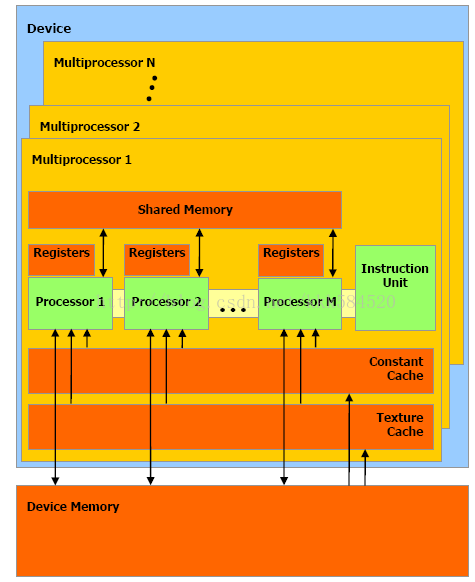
\includegraphics[scale = 0.8]{InfoTransfer.png}
			\end{figure}
			
			从图中可看出,一个\verb|SM|内有\verb|M|个\verb|SP|,\verb|Shared Memory|由这\verb|M|个\verb|SP|共同占有。另外指令单元也被这\verb|M|个\verb|SP|共享,即\verb|SIMT|架构(单指令多线程架构),一个\verb|SM|中所有\verb|SP|在同一时间执行同一代码
			
			为了实现线程通信,仅仅靠共享内存还不够,需要有同步机制才能使线程之间实现有序处理。通常情况是这样:当线程A需要线程B计算的结果作为输入时,需要确保线程B已经将结果写入共享内存中,然后线程A再从共享内存中读出。同步必不可少,否则,线程\verb|A|可能读到的是无效的结果,造成计算错误。同步机制可以用\verb|CUDA|内置函数:\verb|__syncthreads()|;当某个线程执行到该函数时,进入等待状态,直到同一线程块(\verb|Block|)中所有线程都执行到这个函数为止,即一个\verb|__syncthreads()|相当于一个线程同步点,确保一个\verb|Block|中所有线程都达到同步,然后线程进入运行状态。
			
			\begin{lstlisting}[frame = ]
	//Begin   
	if this is thread B   
		write something to Shared Memory;   
	end if   
	__syncthreads();   
	if this is thread A   
		read something from Shared Memory;   
	end if   
	//End   
			\end{lstlisting} 
			
			\subsection{线程通信实例}
			
				\begin{figure}[hb]
					\centering
					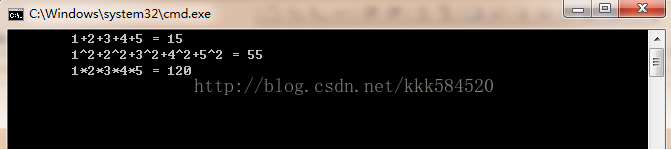
\includegraphics[scale = 0.8]{ExampleInfo.png}
				\end{figure}
				
			很简单,就是分别求出1~5这5个数字的和,平方和,连乘积。相信学过C语言的童鞋都能用\verb|for|循环做出同上面一样的效果,但为了学习\verb|CUDA|共享内存和同步技术,我们还是要把简单的东西复杂化。 
			
			简要分析一下,上面例子的输入都是一样的,1,2,3,4,5这5个数,但计算过程有些变化,而且每个输出和所有输入都相关,不是前几节例子中那样,一个输出只和一个输入有关。所以我们在利用\verb|CUDA|编程时,需要针对特殊问题做些让步,把一些步骤串行化实现。
			 
			输入数据原本位于主机内存,通过\verb|cudaMemcpy API|已经拷贝到\verb|GPU|显存(术语为全局存储器,\verb|Global Memory|),每个线程运行时需要从\verb|Global Memory|读取输入数据,然后完成计算,最后将结果写回\verb|Global Memory|。当我们计算需要多次相同输入数据时,大家可能想到,每次都分别去\verb|Global Memory|读数据好像有点浪费,如果数据很大,那么反复多次读数据会相当耗时间。索性我们把它从\verb|Global Memory|一次性读到SM内部,然后在内部进行处理,这样可以节省反复读取的时间。 
			
			有了这个思路,结合上节看到的SM结构图,看到有一片存储器叫做\verb|SharedMemory|,它位于SM内部,处理时访问速度相当快(差不多每个时钟周期读一次),而全局存储器读一次需要耗费几十甚至上百个时钟周期。于是,我们就制定A计划如下:
 
			\textbf{线程块数}:1,块号为0;(只有一个线程块内的线程才能进行通信,所以我们只分配一个线程块,具体工作交给每个线程完成)
			 
			\textbf{线程数}:5,线程号分别为\verb|0~4|;(线程并行,前面讲过)
			 
			\textbf{共享存储器大小}:5个\verb|int|型变量大小(\verb|5 * sizeof(int)|)。 
			
			\textbf{步骤一}:读取输入数据。将\verb|Global Memory|中的5个整数读入共享存储器,位置一一对应,和线程号也一一对应,所以可以同时完成。
			 
			\textbf{步骤二}:线程同步,确保所有线程都完成了工作。 
			
			\textbf{步骤三}:指定线程,对共享存储器中的输入数据完成相应处理。
			
			\begin{lstlisting}
	__global__ void addKernel(int *c, const int *a)   
	{   
		int i = threadIdx.x;   
		extern __shared__ int smem[];   
		smem[i] = a[i];   
		__syncthreads();   
		if(i == 0)  // 0号线程做平方和   
		{   
			c[0] = 0;   
			for(int d = 0; d < 5; d++)   
			{   
				c[0] += smem[d] * smem[d];   
			}   
		}   
		if(i == 1)//1号线程做累加   
		{   
			c[1] = 0;   
			for(int d = 0; d < 5; d++)   
			{   
				c[1] += smem[d];   
			}   
		}   
		if(i == 2)  //2号线程做累乘   
		{   
			c[2] = 1;   
			for(int d = 0; d < 5; d++)   
			{   
				c[2] *= smem[d];   
			}   
		}   
	}   
	
	addKernel<<<1, size, size * sizeof(int), 0>>>(dev_c, dev_a);
			\end{lstlisting}
	\section{编译}
		设备程序需要由\verb|NVCC|进行编译,而主机程序只需要由主机编译器(如\verb|VS2008中的cl.exe,| \verb|Linux上的GCC|)。\textbf{主机程序}主要\textit{完成设备环境初始化},\textit{数据传输等必备过程},\textbf{设备程序}\textit{只负责计算}。 
		
		\subsection{编译注意事项}
			\url{http://blog.csdn.net/shengwenj/article/details/48917203}		
\end{document} 
 		    